\documentclass[11pt]{article}
\usepackage[a4paper,margin=2.3cm]{geometry}
\usepackage[T1]{fontenc}
\usepackage{lmodern}
\usepackage{amsmath}
\usepackage{graphicx}
\usepackage{booktabs}
\usepackage{siunitx}
\usepackage[numbers,sort&compress]{natbib}
\usepackage[hidelinks]{hyperref}
\graphicspath{{figures/}{../figures/}}

\title{Knowing when not to trust it: band gaps of two-dimensional semiconductors\\
with a calibrated verdict, audited labels and pre-registered experiments}
\author{Danil Balandin\\[2pt]
\small National Research University of Electronic Technology (MIET), Moscow\\
\small Electronics and Nanoelectronics, Department of Integrated Circuit Design and Architecture}
\date{October 2026}

\begin{document}
\maketitle

\begin{abstract}
Machine-learned band gaps are cheap enough to screen tens of thousands of candidate
monolayers, but a number alone does not say when it should not be used. We describe
NanoMatAI, an open tool that predicts the PBE band gap of a two-dimensional layer from
its structure and attaches to every prediction a verdict (reliable, check or
out-of-domain) and a calibrated 90\% interval. A five-member CGCNN ensemble with a
per-atom bond-angle descriptor, trained on 45\,857 PBE monolayers from Alexandria,
2DMatPedia and MC2D, reaches a mean absolute error of 0.190\,eV (95\% CI 0.173--0.209)
on a test set whose compositions never occur in training, against 0.430\,eV for a
composition model on the same set; on predictions it marks reliable the error is
0.10\,eV. The verdict combines a five-seed metal/semiconductor gate, the ensemble
spread and the cosine distance to the training set in the model's latent space; it
orders the error on held-out data from four databases, including C2DB and JARVIS, on
which the regressor never trained; on C2DB the error is 0.25\,eV overall. Every change
to the model was decided by a rule written before training and judged against a
control retrained in the same session; seven of the last eight such experiments failed
their rule and were not shipped. Auditing the data
structure by structure found incorrect labels in Alexandria's planar honeycombs and
59 layers whose labels disagree between cells of the same structure, and measured the
spin-orbit offset between databases. We also report eight errors of protocol made and
corrected during the project, and a test of ten language models given the tool over
the Model Context Protocol. Code, weights, data splits and a browser predictor that
agrees with the Python package to within $10^{-5}$\,eV are public.
\end{abstract}

\section{Introduction}

Two-dimensional semiconductors are candidates for transistor channels, photodetectors
and light emitters, and the first number one asks of a candidate layer is its band gap.
Density-functional databases now hold tens of thousands of monolayers: Alexandria 2D
\citep{alexandria2d}, C2DB \citep{c2db2018,c2db2021}, 2DMatPedia \citep{2dmatpedia},
MC2D \citep{mc2d2018,mc2d2023} and JARVIS \citep{jarvis}. Graph neural networks trained on
such data predict gaps of new structures in milliseconds \citep{cgcnn,alignn}, and
machine-learned 2D gaps have been reported many times \citep{review2d}. What these
predictions rarely
come with is a statement of when not to use them. A screen over thousands of
hypothetical layers is exactly where a model meets chemistry it has not seen, and a
confident wrong number there is worse than none.

This paper does not claim a new architecture or a better error on a shared benchmark;
no shared benchmark for 2D band gaps exists. Its contributions are:
\begin{enumerate}
\item A band-gap predictor for monolayers whose every output carries a verdict and a
  calibrated interval, built from three independent out-of-domain signals, with the
  interval calibrated per population (Section~\ref{sec:trust}).
\item A sequence of data and architecture experiments, each judged by a rule written
  before training against a same-session control, including the ones that failed
  (Section~\ref{sec:experiments}).
\item A structure-by-structure audit of four databases that finds and flags incorrect
  labels and measures the offsets between methods (Section~\ref{sec:audit}).
\item An account of eight errors of protocol, all of the kind ``two numbers that were
  not measured the same way'', and how each was caught (Section~\ref{sec:protocol}).
\item A public tool: a browser predictor, a precomputed table of 28\,372 layers, a
  Python package and a language-model interface (Section~\ref{sec:tool}).
\end{enumerate}

\section{Data}\label{sec:data}

\paragraph{Target.} The regression target is the PBE \citep{pbe} band gap without
spin-orbit coupling (SOC), the level of Alexandria 2D. Only semiconductors
($E_g > 0.01$\,eV) are regressed; metals are the job of a separate gate.

\paragraph{Training set.} The stable set is the 13\,349 Alexandria monolayers within
0.1\,eV/atom of the convex hull. It is split by reduced formula into training (10\,733),
validation (1\,290) and test (1\,326) with \texttt{GroupShuffleSplit}; validation and test
have not changed since the first model, so every generation is scored on the same
1\,326 structures. Four pre-registered experiments
(Section~\ref{sec:experiments}) grew the training set to 45\,857 monolayers: 32\,736
metastable Alexandria layers up to 1.0\,eV/atom above the hull, 1\,646 non-magnetic
2DMatPedia layers and 742 MC2D layers that have no structural twin in Alexandria and
contain none of V, Cr, Mn, Fe, Co, Ni. No added formula occurs in the validation or test
split or in any held-out set below.

\paragraph{Held-out populations.} Besides the stable test set (T\textsubscript{alex}),
each experiment held out sets by formula from the data it added: metastable Alexandria
at 0.1--0.2 (T\textsubscript{meta}, 2\,512), 0.2--0.5 (T\textsubscript{far}, 2\,524) and
0.5--1.0\,eV/atom (T\textsubscript{vfar}, 453), non-magnetic 2DMatPedia
(T\textsubscript{2dmp}, 397) and MC2D (T\textsubscript{mc2d}, 273). The model never
trained on C2DB or JARVIS dft\_2d; their 1\,115 and 696 semiconductors in the screening
table serve as external sets, with the caveat that their labels are PBE with SOC (C2DB)
and OptB88vdW (JARVIS).

\section{Model}\label{sec:model}

The regressor is CGCNN \citep{cgcnn} in PyTorch Geometric \citep{pyg}: atomic numbers
embedded in 128 dimensions, four \texttt{CGConv} layers over periodic neighbours within
8\,\AA{} whose edges carry the distance expanded in 40 Gaussians, mean pooling and a
two-layer head. A distance-only graph barely separates polymorphs of one composition:
on 1H against 1T-MX\textsubscript{2} the first model compressed a 0.44\,eV DFT
difference into 0.12\,eV. Each atom therefore also carries a 9-bin soft histogram of
the cosines of its bond angles within 4\,\AA, weighted by a smooth cutoff and
normalised; against its own control this lowered the test error from 0.271 to
0.246\,eV (paired difference 0.026\,eV, 95\% bootstrap interval 0.015--0.037, Wilcoxon
$p = 4\times10^{-5}$) and roughly doubled the separation of 1H from 1T.

A layer whose vacuum is thinner than the cutoff would gain edges to its own periodic
image, so both training and inference pad the vacuum to 20\,\AA{} when it is below
9\,\AA; a structure with no gap of at least 5\,\AA{} along any axis is flagged as not a
2D layer. The ensemble has five members (seeds 0--4), trained up to 200 epochs with
early stopping on the validation split.

The composition baseline is a random forest on Magpie features \citep{magpie}, scored on
the identical split.

\section{The trust layer}\label{sec:trust}

\paragraph{Three signals.} (i) A metal/semiconductor gate: a five-seed classifier
ensemble with the same trunk, trained on 93\,238 Alexandria, 2DMatPedia, C2DB and
JARVIS layers, metals included, ROC-AUC 0.984 on its stable test and 0.917--0.951 on the held-out
populations, with its threshold (0.47) chosen on validation. Mixing functionals is
allowed for this binary label only. (ii) The ensemble spread. Members trained on the
same data agree for the wrong reason where a chemistry is represented once; the spread
measures disagreement between initialisations, not coverage. (iii) The latent
distance: one minus the mean cosine similarity of a structure's pooled embedding to its
ten nearest training embeddings, the metric proposed by \citet{janet2019}. On the test
set the spread and the distance correlate with the absolute error at Spearman 0.445
and 0.429, and their product at 0.481.

\paragraph{Verdict.} A prediction is out-of-domain if the gate calls it a metal, if it
is not a layer, if its spread is above the validation 75th percentile, or if its latent
distance is above the validation 90th percentile; it is check if its spread is above
the median or its distance above the 75th percentile; otherwise reliable. On the test
set the three tiers hold 43, 28 and 29\% of the structures with mean absolute errors of
0.098, 0.141 and 0.375\,eV.

\paragraph{Calibrated interval.} Raw ensemble spreads cover the error at $\pm1\sigma$
46\% of the time, the overconfidence usually found for ensembles \citep{tran2020}, so
the spread is scaled. A single factor fitted on validation (3.77
for 90\%) covers 91.6\% of the test set but only 84\% of held-out metastable layers,
and neither the spread nor the distance sees the difference. A logistic head on the
concatenated member embeddings separates metastable from near-hull training structures
at ROC-AUC 0.911 on held-out data; the interval scale is then read from a cell of
(resembles metastable, spread quartile). Over 20 random halvings of T\textsubscript{meta}
by formula, the coverage of the held-out half rose from 84.0 to 89.6\% while the test
set stayed at 91.5\%. An earlier rule that also demoted reliable predictions resembling
metastable structures was withdrawn: it reversed the order of the reliable and check
tiers on every external population.

\paragraph{Derived quantities.} Ridge heads on the 640-dimensional concatenated
embedding, fitted to C2DB G\textsubscript{0}W\textsubscript{0} and Bethe--Salpeter results
for 199 non-magnetic monolayers, give a quasiparticle gap, the exciton binding energy
and an optical gap (direct G\textsubscript{0}W\textsubscript{0} gap minus binding energy),
with composition-disjoint cross-validated errors of 0.236, 0.139 and 0.220\,eV. A
second ensemble trained on C2DB's work function (test MAE 0.254 against 0.314 for
composition) places the band edges at the work function $\pm$ half the gap, with its own
verdict; edges are shown only when both models accept the structure.

\section{Pre-registered experiments}\label{sec:experiments}

Every change was decided by a rule written into the script header before training. A
candidate arm had to stay within $+0.005$\,eV of a control retrained in the same
environment on T\textsubscript{alex}, with the upper end of the paired 95\% bootstrap
interval below $+0.015$, and to improve a population it targeted with the whole interval
below zero, while no held-out set got worse with its whole interval above zero. Two
trainings of one recipe in different environments differ by about 0.005--0.01\,eV, which
is why comparisons are always against a same-session control.

\begin{table}[t]
\centering
\caption{Data experiments: mean absolute error (eV) of the same-session control and of
the candidate arm, on the stable test set and on the held-out set the step targeted,
with the paired difference on the latter. Each row is a separate session whose control
is the recipe shipped before it; all four arms passed their rules and shipped.
Metastable bands are in eV/atom above the hull.}
\label{tab:experiments}
\small
\begin{tabular}{lccc}
\toprule
added to training & T\textsubscript{alex} & target set & paired diff.\ (95\% CI) \\
\midrule
metastable $\le$0.2 and 2DMatPedia & 0.249 $\to$ 0.225 & T\textsubscript{2dmp} 0.770 $\to$ 0.437 & $-0.333$ ($-0.406$, $-0.261$) \\
metastable 0.2--0.5 & 0.230 $\to$ 0.197 & T\textsubscript{far} 0.438 $\to$ 0.256 & $-0.182$ \\
metastable 0.5--1.0 & 0.191 $\to$ 0.186 & T\textsubscript{far} 0.256 $\to$ 0.248 & $-0.007$ ($-0.012$, $-0.002$) \\
MC2D & 0.191 $\to$ 0.190 & T\textsubscript{mc2d} 0.449 $\to$ 0.385 & $-0.064$ ($-0.103$, $-0.027$) \\
\bottomrule
\end{tabular}
\end{table}

\paragraph{Metastable data helped.} Early models used only the stable set, because a
model trained to 0.2\,eV/atom had scored worse (0.262 against 0.215). Those two numbers
were measured on different test sets, the second half metastable. On a fixed test set
the metastable data improved every population (Table~\ref{tab:experiments}); the return
ran out at 1\,eV/atom (0.004\,eV on T\textsubscript{alex}). Within compositions, the
model now separates polymorphs much better: on C2DB the ratio of predicted to DFT
spread within a composition rose from 0.37 to 0.87 over the project, and for 1H
against 1T pairs from 0.18 to 0.75, with the sign right for 92\% of pairs.

\paragraph{Experiments that failed.} The following were tested under the same kind of
rule and did not ship: bagged ensemble members (the spread became more honest on sparse
chemistry, with Spearman 0.45 $\to$ 0.50, but accuracy fell by 17\% and the combined
signal barely moved); a three-way gap-type answer (direct, indirect, too close to call);
a learned error head as a fourth trust signal; a three-body edge update (worse on
T\textsubscript{alex} by 0.010\,eV, 95\% CI 0.002--0.018); effective-mass models on the
full C2DB release (structure did not beat composition, $\log_{10}$ errors 0.267 against
0.252 for electrons); and ridge heads for the SOC shift and for HSE06 gaps on the
frozen latent space. The last two beat their baselines on average but gave tungsten
dichalcogenides less than half of their spin-orbit shift (WS\textsubscript{2}
$-0.14$\,eV against C2DB's $-0.28$), a failure we attribute to a latent space trained
on SOC-free labels.

\section{Auditing the databases}\label{sec:audit}

\paragraph{Matching layers.} Comparing databases by formula mixes different
polymorphs: 2DMatPedia and Alexandria agree to 0.44\,eV by formula but 0.09\,eV by
structure. Structure matching of slabs has its own trap: pymatgen's
\texttt{StructureMatcher} normalises its site tolerance by $(V/N)^{1/3}$, and in a slab
$V$ is mostly vacuum, so a tolerance of 0.1 is about 0.5\,\AA{} and a planar and a
buckled layer match. We bring every layer to one frame (vacuum along the normal,
primitive cell), use \texttt{ltol}~=~\texttt{stol}~=~0.1 without scaling, and require
the layer thicknesses to agree within 0.2\,\AA. On 1\,131 shared layers, Alexandria and
2DMatPedia then agree to a median of 0.0014\,eV/atom in energy and to a mean absolute
0.088\,eV in gap (median 0.055, Pearson 0.995); MC2D agrees with Alexandria to 0.070\,eV on 317 layers, but compounds
of the magnetic 3d metals disagree by 0.374\,eV against 0.057 for the rest.

\paragraph{Incorrect labels.} Alexandria labels planar graphene 1.23\,eV in a 2-atom
cell and 1.13\,eV in a 4-atom cell, against zero in C2DB, 2DMatPedia and JARVIS; planar
silicene 0.86 against zero; and one layer of boron phosphide 1.31\,eV in its 2-atom
cell against 0.91\,eV in its 4-, 6- and 8-atom cells, at the same energy. In a
$\sqrt3\times\sqrt3$ cell the K point folds onto $\Gamma$, which suggests a k-point grid
that misses K. More generally, 59 structures stored in several Alexandria cells carry
labels more than 0.1\,eV apart. These 143 labels are flagged in the released data,
excluded from error statistics and marked wherever a prediction cites them.
2DMatPedia, in turn, is about 1\,eV high on the ZrNCl family at identical structure and
energy.

\paragraph{Methods.} Against C2DB, whose gaps include SOC, the model's predictions for
compounds of elements with $Z\ge52$ come out 0.27\,eV high on average and the rest
0.03\,eV; against held-out Alexandria there is no such offset. All of the shortfall in
interval coverage on C2DB (82\% against 90\% on Alexandria) sits in the heavy-element
compounds. In C2DB's own numbers the Fermi level lies exactly mid-gap, so the work
function $\pm$ half the gap is C2DB's definition of the band edges; against those edges
the tool's are off by 0.15\,eV where shown, 0.20\,eV where the work-function model never
trained, and 0.28--0.31\,eV where the rule withholds them.

\section{Results}\label{sec:results}

\begin{figure}[t]
\centering
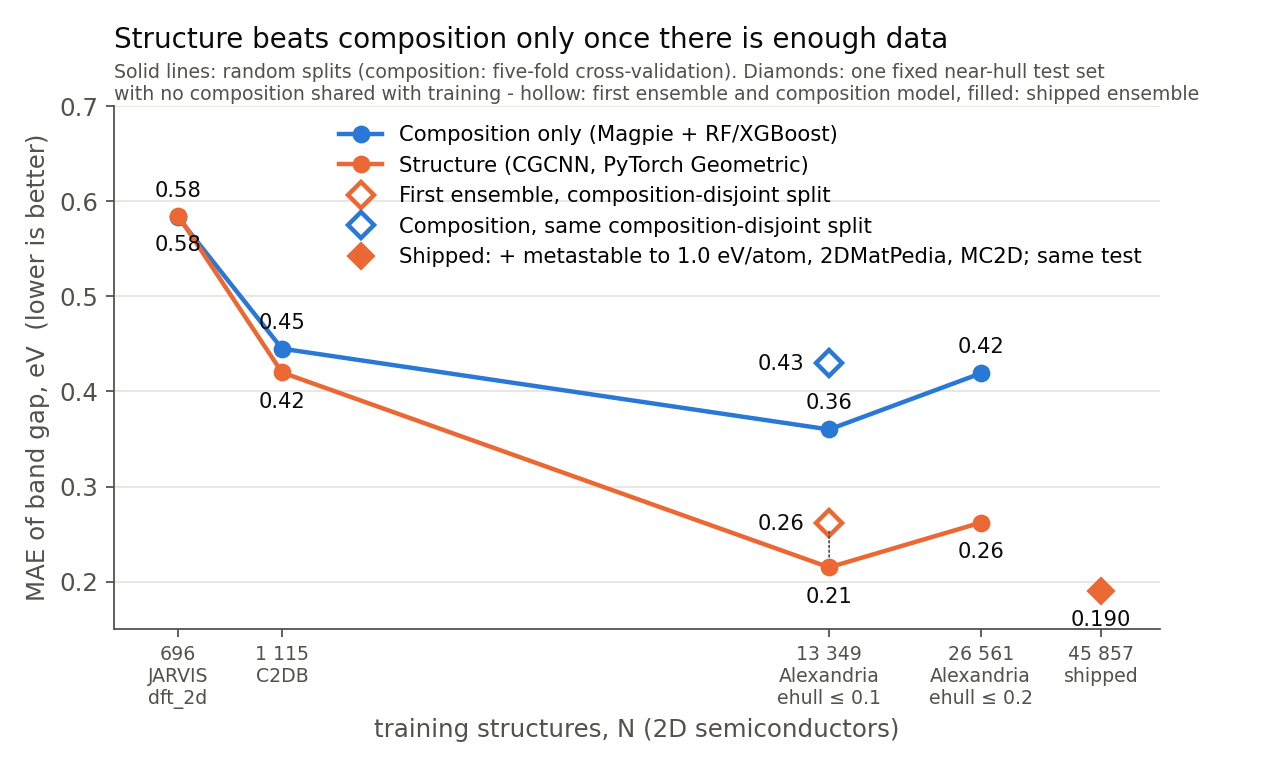
\includegraphics[width=0.8\linewidth]{mae_vs_n.png}
\caption{Test error against the number of training structures. Solid lines: the early
experiments as first measured, on random splits, with the composition model scored by
five-fold cross-validation. Diamonds: the fixed composition-disjoint test set, on which
the composition model scores 0.430\,eV, the first ensemble 0.261\,eV and the shipped
ensemble 0.190\,eV.}
\label{fig:scaling}
\end{figure}

On the stable test set the ensemble's error is 0.190\,eV (95\% CI 0.173--0.209), RMSE
0.395, $R^2$ 0.916, against 0.430\,eV for the composition baseline on the identical set
(Fig.~\ref{fig:scaling}). In the early random-split experiments the two were level
with 696 structures, the structure model was ahead by about 5\% with 1\,115, and from
13\,349 on it was decisively ahead.

On the external sets the verdict keeps its order: mean errors over the reliable, check
and out-of-domain tiers are 0.127/0.191/0.337\,eV on held-out Alexandria,
0.178/0.212/0.350 on C2DB, 0.307/0.356/0.487 on JARVIS and 0.153/0.289/0.544 on held-out
MC2D. On C2DB, which the model never trained on, the error is 0.246\,eV overall and
0.189\,eV over the 720 structures it does not disown. The 90\% interval covers 87.9\% of
the 6\,625 rows of the screening table the model never trained on: 90.5\% on Alexandria,
82.3\% on C2DB and 78.3\% on JARVIS, the last two partly the difference in method.

For comparison, and with the caveat that datasets and protocols differ: the Gap2D model
of Uni2D \citep{uni2d} reports 0.53\,eV in 20-fold cross-validation on C2DB itself; on the
three-dimensional \texttt{matbench\_mp\_gap} task \citep{matbench} with random splits,
the best graph networks reach about 0.16--0.18\,eV.

\begin{figure}[t]
\centering
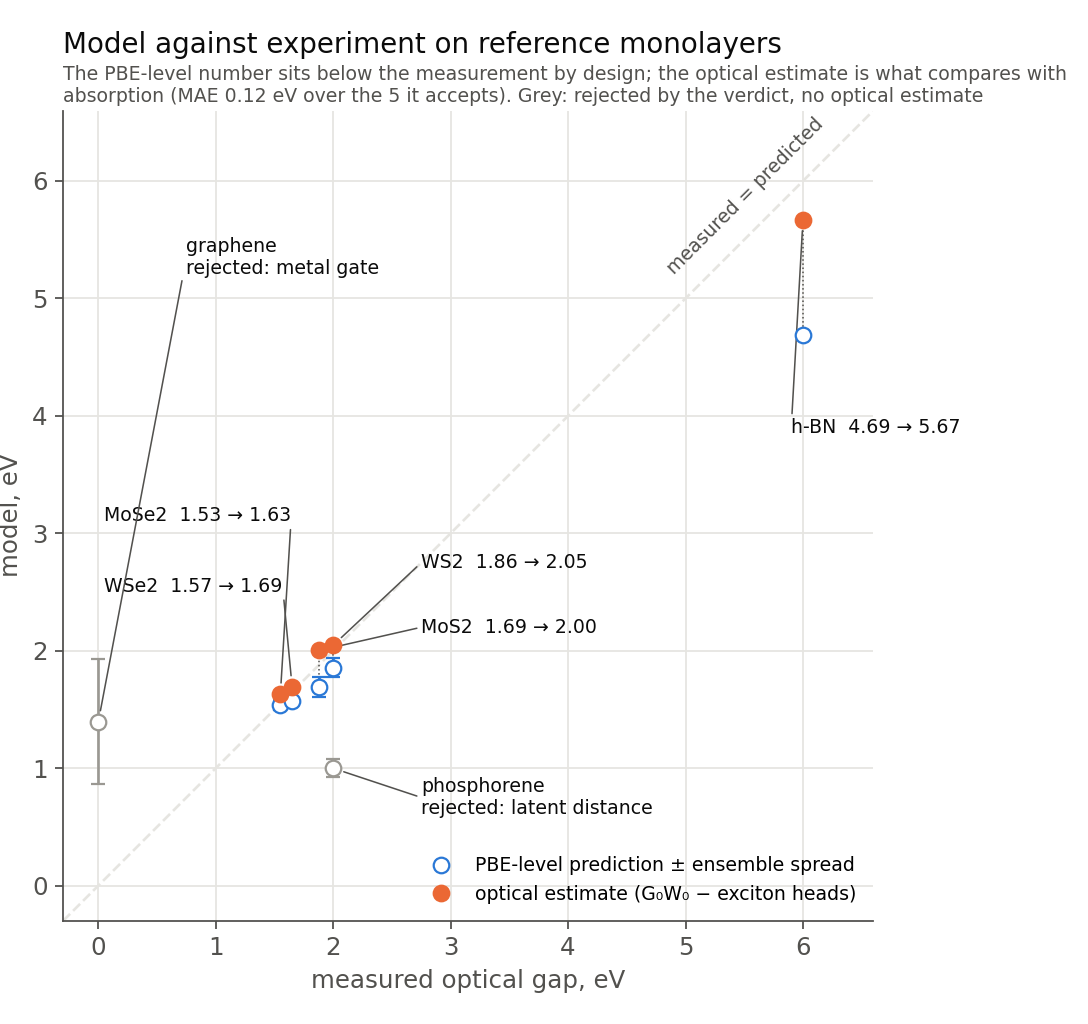
\includegraphics[width=0.62\linewidth]{experiment_validation.png}
\caption{Seven reference monolayers: the PBE-level prediction (open) and the optical
estimate from the latent heads (filled) against measured optical gaps. Graphene,
stopped by the metal gate, and phosphorene, stopped by the latent distance, are
rejected and get no optical estimate.}
\label{fig:experiment}
\end{figure}

Against experiment, the optical estimate places monolayer MoS\textsubscript{2} at
2.00\,eV against a measured 1.88\,eV (Fig.~\ref{fig:experiment}); the estimate is
trained on G\textsubscript{0}W\textsubscript{0} and Bethe--Salpeter results, and over
the five measured monolayers it accepts it is off by 0.12\,eV on average, too few
points for more than a sanity check. Graphene is rejected by the metal gate and
phosphorene by the latent distance.

\section{Errors of protocol}\label{sec:protocol}

Eight conclusions in this project were wrong because two numbers were not measured the
same way. We list them because each is easy to repeat.
\begin{enumerate}
\item A composition baseline scored by five-fold cross-validation (0.360\,eV) was set
  against a network scored on a composition-disjoint split; on the same split the
  baseline scores 0.430, so the network's advantage was 39\%, not 27\% (now 56\%).
\item ``Metastable structures hurt training'' came from two models scored on different
  test populations (Section~\ref{sec:experiments}).
\item The latent-distance signal was motivated by phosphorene, ``0.82\,eV predicted,
  2.0 measured, rated reliable''. That compared a PBE gap with an optical measurement;
  phosphorene's PBE gap is 0.85--0.90\,eV in every database, and the structure was in
  the training set. The signal stands on its statistics, not on the anecdote.
\item A held-out set described as composition-disjoint from all training was disjoint
  only from the added data; 40\% of it were polymorphs of training formulas.
\item The structure matcher's tolerance admitted different polymorphs as twins, so two
  of five ``incorrect labels'' first reported for Alexandria were different structures.
\item The external check on 2DMatPedia and, later, on MC2D excluded only Alexandria
  twins after those databases had themselves entered training.
\item A difference of two corrections fitted on the same four TMDs was read as the
  exciton binding energy; the agreement was circular.
\item Band edges were reported within 0.15\,eV of unattributed literature values, which
  sit above the PBE level; part of the agreement was the missing SOC.
\end{enumerate}

\section{The tool}\label{sec:tool}

The precomputed table of 28\,372 layers (Alexandria to 0.2\,eV/atom, C2DB, JARVIS) is
served as a static page with filters by gap, elements, verdict and intended use, a
periodic-table map of the error on unseen structures, and a view by prototype. A
JavaScript port of the predictor runs in the browser on a user's CIF or POSCAR; on
2\,016 structures from four databases, a quarter as symmetrised CIF, it agrees with the
Python package to \SI{2e-6}{eV} in the gap with no verdict differing, and takes about
60\,ms per structure once the 34\,MB of weights have loaded. Each prediction names its
nearest training structures with their labels, so a number that largely recalls a known
layer is not mistaken for a new one. An MCP server exposes the tool to language models
with the verdict first. Ten models, seven open (3.8--31\,B parameters) and three from
the Claude family, answered eight questions with a trap in each, in three runs between
which only the tool's output changed; this raised the open models from 64 to 75 of 112
points, while invented
citations and photon-energy-to-colour conversions were not fixed by anything the tool
returned.

\section{Limitations}

The target is PBE without SOC, so gaps of heavy-element compounds are high against SOC
references by about 0.27\,eV, and absolute gaps are underestimated against experiment.
Learning the SOC and hybrid-functional levels jointly with PBE in one network, as
multi-fidelity models do \citep{chen2021}, would address this; it is untested here.
The interval is calibrated on Alexandria and covers less of populations computed with
other methods. Light main-group chemistry remains the weakest. The gap-type classifier
is reliable for direct calls (92\%) but not for indirect ones (35\%). One ensemble member
fails on molecular fluorine layers, which the ensemble disowns. The prediction assumes
a relaxed structure; an experimental cell 2\% larger moves the gap and can trip the gate.

\section*{Data and code availability}

Code, weights, splits, flags and the precomputed table:
\url{https://github.com/ac1esan/nanomat-ai} (MIT licence; C2DB-derived files CC BY-NC
4.0). The release described here, v1.5.0:
\url{https://doi.org/10.5281/zenodo.23453267}; all releases:
\url{https://doi.org/10.5281/zenodo.22863467}. Browser:
\url{https://ac1esan.github.io/nanomat-ai/}.

\bibliographystyle{unsrtnat}
\bibliography{refs}

\end{document}
